\chapter{Available high-throughput normal human Datasets}
\label{ch:datasets}

\begin{comment}
\setlength{\epigraphwidth}{0.57\textwidth}
\setlength{\epigraphrule}{0.1pt}
\epigraph{Data! Data! Data! I can’t make bricks without clay!}{Sherlock Homes
    (Sir Arthur Conan Doyle)}
\end{comment}

In this chapter, I describe the data used within my project.

\section{Introduction}

Every dataset with which I worked is fitting three main criteria.
They comprise human normal samples from at least three kind of tissues.
They are untargeted high-throughput; either sequenced with \Rnaseq\
for the transcriptomic studies or
analysed with Mass spectrometry for the proteomic ones.
Finally, the \emph{raw} data is available and reusable.


\section{Transcriptomics}

There are a few more studies that I wanted to use on the
transcriptomic side, but the last previous point was often the critical reason
why they have not been included.

Indeed, many times I encountered data with ambiguous encoding format and, as the
studies were a little bit outdated,
I also could not get the information from the original authors.
I describe hereafter the 5 transcriptomic datasets I used
in the chronological order of their first public release.
The \cref{tab:Trans5DF} summarises the main characteristics of the different
datasets.

\begin{sidewaystable}
           \centering
           \caption{\label{tab:Trans5DF}General description of the 5 transcriptomic
           dataset (\Rnaseq) used for this study}
       \begin{tabular}{@{}cccccccccc@{}}
       \toprule
       \multicolumn{1}{c|}
           {\multirow{2}{*}{ArrayExpress ID}} &
            \multicolumn{1}{c|}{\multirow{2}{*}{Data ID}} &
            \multicolumn{2}{c|}{\begin{tabular}[c]{@{}c@{}}Library\\Preparation\end{tabular}} &
            \multicolumn{2}{c|}{Sequencing} &
            \multicolumn{2}{c|}{Replicates} &
            \multicolumn{1}{c|}{\multirow{2}{*}{\begin{tabular}[c]{@{}c@{}}Tissue\\
                    Number\end{tabular}}} &
            \multirow{2}{*}{\begin{tabular}[c]{@{}c@{}}Multi-sampling\\ from the \\ same
            individual\end{tabular}} \\
            \cmidrule(lr){3-8}
            \multicolumn{1}{c|}{} & \multicolumn{1}{c|}{} &
            \multicolumn{1}{c|}{\begin{tabular}[c]{@{}c@{}}Whole\\ RNA\end{tabular}} &
            \multicolumn{1}{c|}{\begin{tabular}[c]{@{}c@{}}PolyA\\ selected\end{tabular}} &
            \multicolumn{1}{c|}{\begin{tabular}[c]{@{}c@{}}Single\\ end\end{tabular}} &
            \multicolumn{1}{c|}{\begin{tabular}[c]{@{}c@{}}Paired\\ end\end{tabular}} &
            \multicolumn{1}{c|}{Biological} & \multicolumn{1}{c|}{Technical} &
            \multicolumn{1}{c|}{} &  \\
       \midrule
       E-MTAB-305 & Castle & Y &  & Y &  &  &  & 11 &  \\
       E-GEOD-30352 & Brawand &  & Y & Y &  & Y &  & 8 &  \\
       E-MTAB-513 & IBM &  & Y & Y & Y &  & (Y) & 16 &  \\
       E-MTAB-2836 & Uhlén &  & Y &  & Y & Y & Y & 32 &  \\
       E-MTAB-2919 & Gtex  & Y &  &  & Y & Y &  & 54 & Y \\
       \bottomrule
       \end{tabular}
\end{sidewaystable}

\subsection{Castle et al. dataset}

This dataset has been published along with the \paper{\citetitle{castleData}}
by \citet{castleData} who were interested to explore
with sequencing-based technology the whole RNA repertoire. They essentially
focused their study on the non coding part and found that
while \glspl{mRNA} could be highly tissue-specific, \glspl{ncRNA} have generally
greater tissue-specific expression patterns.

They used multiple-donors pooled tissues samples (purchased as total \gls{RNA})
and prepared the 11 libraries following a whole transcriptomic protocol
\citep{Armour:2009}: where nonribosomal \gls{RNA} transcripts are
specifically amplified by \gls{PCR}.

They generated an average of 50 millions sequence reads per tissue
using an Illumina Genome Analyser-II sequencer (single-end).
They trimmed their original reads to 28 \gls{nt}
and released them through EMBL archives (\ENA{ERP000257}
and \ArrayExpress{E-MTAB-305}).

Despite several limitations (lack of replicates, old technology, small reads),
I used this dataset for two main reasons. It is the oldest available \Rnaseq\
data I found that was performed on Human normal tissues and it is comprising
\glspl{ncRNA}.

\subsection{Brawand et al. dataset}

In the corresponding article entitled \paper{\citetitle{VTpaper}},
\citet{VTpaper}~collected 6 organs from 10 different vertebrates:
9 mammalians (including Human) and a bird. They are focused on the
evolution of the mammalian transcriptomes --- while there were existing studies
on the matter, the sequencing approach was then creating new perspectives.

They have biological replicates: one male
and one female for the somatic tissue and two males for the testes samples.
They used a polyA-selected protocol to prepare their 131 libraries (including 23
for \species{Homo sapiens}).
Hence, the samples are largely enriched in protein coding genes.

They generated an average of 3,2 billion reads of 76 base pairs per sample
using an Illumina Genome Analyser IIx (single-end) and they released them
through \gls{GEO} (accession number: GSE30352).
I personally retrieved the data from
\ArrayExpress{E-GEOD-30352}\footnote{ArrayExpress routinely imports
datasets from \gls{GEO} on a weekly basis.}.

\subsection{Illumina Body Map 2.0}
This dataset has been first created in 2010 and released in
2011\footnote{See: \citetitle{ibmEnsembl} - \cite{ibmEnsembl}} by Illumina
mostly to advertise its most recent technology improvement at that time:
the paired-end sequencing.
Until then, all the sequencing was done from only one end of the \gls{DNA} (or
\gls{cDNA}) fragments\footnote{Most of the following transcriptome
studies based on \Rnaseq\ are using paired-end sequencing.}.

The first published paper to analyse this dataset was done by
\citet{ibmrelatedpaper}: \paper{\citetitle{ibmrelatedpaper}}.
It was referenced many times since then as it was for a couple of years
the most extensive freely available \Rnaseq\ dataset of human tissues.

It comprises 16 tissues (one donor per tissue), which were prepared with a
polyA-selected library preparation protocol and then have been sequenced once
with a singled-end protocol and then a second time with a paired-end one. There
are some added libraries which have been created by mixing together the 16 tissues.
While each sample has been sequenced twice and that we have in principal
\emph{technical} replicates, these are not ``regular'' technical
replicates\footnote{\emph{Technical} replicates,
by contrast to \emph{biological} replicates,
usually imply that the same sample source and protocols have been used so the
error and the noise of a technique could be determined.}.

The sequencing was performed with an Illumina HiSeq 2000 and the reads were
released through \ArrayExpress{E-MTAB-503} (\ENA{ERP000546}).


\subsection{Uhlén et al. dataset}

The first version of this dataset (\ArrayExpress{E-MTAB-1733}) was published
as a part of \paper{\citetitle{Uhlen2014}} by \citet{Uhlen2014}. Then an extended
version (\ArrayExpress{E-MTAB-2836}), with new samples and 5 new tissues,
was released along with \paper{\citetitle{Uhlen2015}} \citep{Uhlen2015}.
Both papers are part of the
\href{http://www.proteinatlas.org/}{Human Protein Atlas}\footnote{%
\href{http://www.proteinatlas.org/}{http://www.proteinatlas.org/}}.
Uhlén et al.\ have created
an atlas revolving mostly around the spatial distribution of the proteins through
the Human body. They use many approaches and techniques which also include \Rnaseq.

They found that almost half of the proteins are expressed in all analysed tissues
(with an enrichment for the metabolism enzymes).

There are \emph{technical} and \emph{biological} replicates for the 32 tissues.
Except very few cases, the somatic tissues have male and female donors.

The 200 libraries have been prepared following a polyA-selected protocols and
have been sequenced (paired-end) with an Illumina HiSeq 2000 or 2500.

I started to work with the first version, and when the extended version was
released, I included the new samples and tissues to my work.

\subsection{GTEx data}

The Genotype-Tissue Expression (\gls{GTEx}) project is funded by the NIH Common
Fund and aims to establish a resource database and associated tissue bank
for the study of the relationship between genetic variation and gene expression
and other molecular phenotypes in multiple reference tissues. The project was first
explained in a paper from the \cite{GTEx2013}: it consists to quickly collect
many tissues from postmortem donors so genotype-tissue expression analyses could
be done, notably \gls{eQTL} variants studies which study the modulation
of \gls{RNA} expression in function of \glspl{SNP}. The results of the
analyses are released through the GTEx portal (%
\href{http://gtexportal.org}{http://gtexportal.org}). The issue 6235 of
\emph{Science} comprises
many articles from this project. The most relevant to my work is
\paper{\citetitle{GTExTranscript}} from \cite{GTExTranscript}. While they study
the landscape of expression through the different tissues across the donors, they
put emphasis on the variation inter- and intra-individuals across the tissues.

As the project is quite ambitious and the collection and sequencing of the samples
are taking time, several freezes of the data have been released. My work is
including samples up to the fourth release of the pilot phase (v.1.4). This
release includes 54 tissue/cell type collected on 551 individuals.
The 3,276 libraries were prepared from whole \gls{RNA} extracts and then sequenced
with a paired-end protocol on Illumina HiSeq 2000/2500 sequencers which produced
an average of 80 million reads.

The raw data is available for privacy reasons only through controlled access via
\dbGaP{phs000424.v4.p1} (access number specific to the version of the data I used
in my study). While getting access can take time, in principal every request for
academic research should be granted.


\section{Proteomics}

In the issue 7502 of \textit{Nature} (2014), two teams of authors released their
own \emph{``draft of the human proteome''} based on the study of several tissues
with \ms. There were already other human protein maps available,
e.g.\ the Human protein atlas\footnote{%
\href{http://www.humanproteomemap.org/}{www.proteinatlas.org/}}, but those one
were mostly reporting the spatial expression of the proteins (as they were based
on immunohistochemistry or other means of identification) than
quantifying their (non-targeted) abundance in each tissue.


\subsection{Pandey data}

\cite{PandeyData} created the Human Proteome Map\footnote{%
\href{http://www.humanproteomemap.org/}{\small www.humanproteomemap.org/}} which
they released along their paper \paper{\citetitle{PandeyData}}.

To create their map, they have processed 30 kind of histological normal human
tissues and cell line (17 adult tissues, 7 fetal tissues and 6 haematopoietic
cell types) samples. The samples were created from pooled samples of three
individuals (generally two males and one female).

They used a label-free method of library preparation to quantify as many proteins
they could.

They first fractionated the samples to protein level by
\gls{SDS-PAGE} and then at peptide level by \gls{RPLC} to create 85 experimental
samples. Then, they use
state-of-art \gls{MS/MS} protocols (with high-resolution and high accuracy
\glspl{FTMS}: Thermo Scientific Orbitrap instruments).
They generated about 25 million of (\gls{HCD})
high-resolution mass spectra which account for 2,212 \gls{LC-MS/MS} profiles.

While their work to generate the data was highly appraise, the identification and
quantification data they provided the community was quite criticised
(e.g.\ see~\cite{Ezkurdia2014-qx}).

The data was downloaded from ProteomeXchange via the PRIDE repository (%
\Pride{PXD000561}).

\subsection{Kuster data}

In their human proteome approach,
\cite{KusterData} combined newly generated \gls{LC-MS/MS} spectrum
data (about 40\%) with already published one
(either from their colleagues or accessible through repositories ---
for the remaining 60\%).
The data comprised 16,857 experiments involving tissues, body fluids and cell
lines. They used all the data they could access from \gls{PTM} to affinity
purification studies.

They reprocessed the whole collection of spectra to maximise proteome coverage
and make it available through their own repositories: ProteomicsDB\footnote{%
\href{https://www.proteomicsdb.org/}{www.proteomicsdb.org/}}.

The subset of data considered in this study is also known as the Human BodyMap
which is the part that was generated (1,087 \gls{LC-MS/MS} profiles)
by the Kuster lab itself.
It comprises 48 experiments covering 36 tissues
(adult and fetal) and cell lines.
They generated about 14 million of (\gls{HCD}/\gls{CID}) spectra from Thermo
Scientific instruments.

The raw data was downloaded from ProteomicsDB (\Proteomicsdb{PRDB000042}).

\subsection{Cutler data}

This data was generated prior to the \dataset{Pandey} and the dataset{Kuster}
data as it was released in 2011 through PeptideAtlas\footnote{%
    \href{http://www.peptideatlas.org/}{www.peptideatlas.org/}}
\citep{PeptideAtlas}.

It was created by Paul Cutler at Roche Pharmaceuticals.
It comprises 10 different tissues (1,618 \gls{CID} Thermo Scientific raw files).

While this data was never published on its own, it has been used in different
other studies; indeed, the \dataset{Cutler} data is one the datasets that
\cite{KusterData} have used in their original study to create ProteomicsDB.

This data was also downloaded from ProteomicsDB (\Proteomicsdb{PRDB000012}).

\section{Constant processing pipelines}

Despite available quantifications for most of the datasets ---
released either by the original authors (directly \citep{Krupp2012},
\citep{Uhlen2015} or  only upon requests \citep{PandeyData})
or by third-parties \citep{BioGPS1}, \citep{EBIgxa},
\citep{Harmonizome} --- I only used data reprocessed from raw files.

Intuitively, we expect that different processing protocols produce
different results.

In fact along my work, I noticed many potential bias sources that impact
\Rnaseq\ outputs. Many of them have since then been reported in the literature;
annotations \citep{annotationDiff},
contamination \citep{contaminationRNAseq},
quality controls \citep{qualityRNAseq} and
mapping and quantifications pipelines \citep{Fonseca2014}
have great effects on the final quantification.

Moreover, the normalisation method of the quantified data also
greatly impacts the final expression values
\citep{Dillies2013}, \citep{normalisation2}.

In facts, the available normalised \Rnaseq\ values are the products
of different methodologies, e.g.\ \citep{GTExTranscript} and \citep{Krupp2012}.
Hence, reprocessing all the transcriptomic datasets was the logical
first step of this study.

Likewise, the proteomic datasets were reprocessed from the raw spectra by Dr
James Wright.


\subsection{Transcriptome raw data processing}

While I downloaded and entirely processed four of the transcriptomic datasets
myself (\dataset{Castle},
\dataset{Brawand},
\dataset{IBM},
\dataset{Uhlén})
it was not the case for the \Gtex\ dataset. Since this
data is involved in many project within the \EBI\ and due to the huge amount of
files and data,
it was agreed that this would be processed centrally by one person and then
redistributed to all the other interested parties. Dr Nuno Fonseca had this
tremendous task and provided me with quantification data,
both for each sample separately and then for each tissue (all relevant samples
pooled together).

For the sake of consistency and to avoid more biases \citep{h38vsh37},
that led me to reprocess all the other four \Rnaseq\ datasets
to comply with the reference used for the \Gtex\ samples. The silver lining
was that they were built with the new reference of the
Human genome GRCh38 (and then annotated with ENSEMBL 76).

In the early stages of my research, I was running each of the different steps
sequentially and manually. While the \EBI\ cluster helped a lot with the
processing of the numerous files,   the many file integrity checks
Fortunately, Dr Nuno Fonseca developed
\irap\footnote{https://nunofonseca.github.io/irap/}, an ``integrated RNA-seq
analysis Pipeline''. This meta-pipeline allows to automatise the

\begin{table}
\centering
\caption[Technical description of the 5 transcriptomic datasets]{%
\label{tab:Lib5DF}\textbf{Technical description of the 5 transcriptomic
    datasets}\\\footnotesize{I processed all the datasets but the one in italic.\\
    For the Brawand dataset, I only processed the \species{Homo sapiens} part.}}
\begin{tabular}{@{}cccc@{}}
\toprule
Dataset             & Sample number (biologic) & Library number & File number \\
\midrule
Castle              & 11                       & 11             & 11          \\
Brawand             & 18                       & 21             & 23          \\
Illumina Body Map   & 16                       & 36             & 48          \\
Uhlén               & 122                      & 200            & 400         \\
    \textit{\color{darkgray}\Gtex\ v.1.4} & \textit{\color{darkgray}3276} &
    \textit{\color{darkgray}3276}      & \textit{\color{darkgray}6552}    \\
\bottomrule
\end{tabular}
\end{table}




\begin{itemize}
        \item all the data RNAseq
        \item has to reprocess several time due to evolution of Annotation
\end{itemize}

First I  was doing it manually and very tedious; but as I was reprocessing the data
as I had access to more data and new ensembl annotations were released, \irap\
was developed by Nuno Fonseca. It is a meta-pipeline which has speeded a lot the
work. Still need a configuration file. But everything follows the same protocol.
Add the final methodology.

I am using only gene levels quantification and not isoforms.

\begin{figure}
    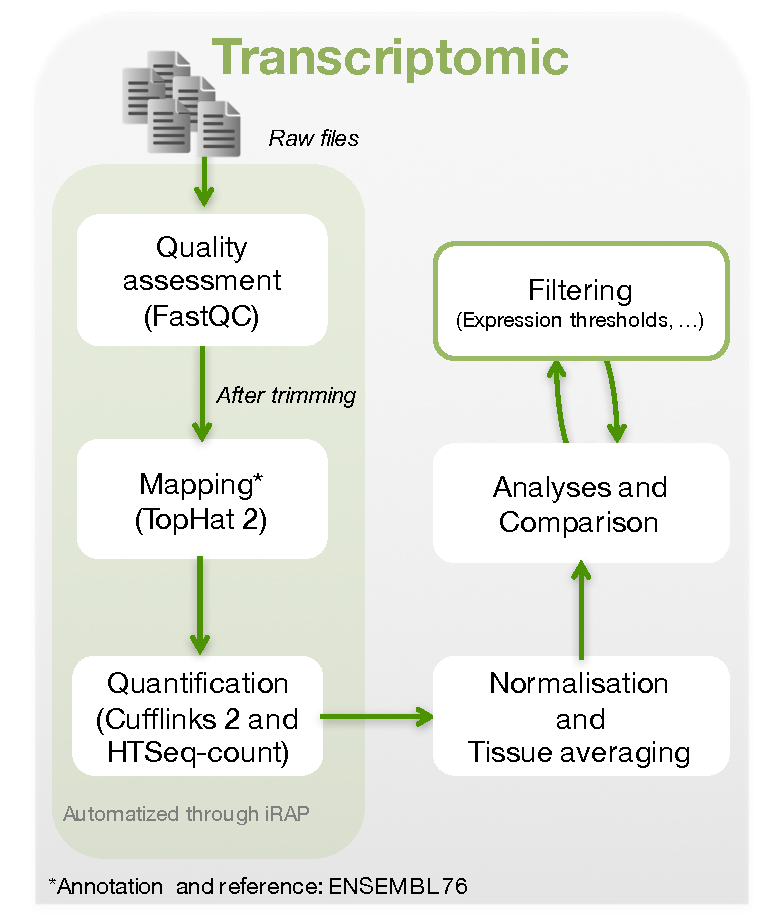
\includegraphics[scale=0.75]{additional/pipelineTrans.pdf}\centering
    \caption[General steps for processing the transcriptomic
    data]{\label{fig:pipelineTrans}\textbf{General steps for processing the
    transcriptome} [TK]}
  \end{figure}


\subsection{Proteome raw data}

Similarly to the transcriptome issue, there is the proteome which is actually
trickier (possible problem with Pandey data analyses). Really depends which
threshold and \gls{FDR} tolerate. And what database and algorithm are used to perform
the identification of the proteins. More messy.

All the data has been processed by James.

Small problem about mapping back proteins to transcripts.



And again describe the methodology.

  \begin{figure}
      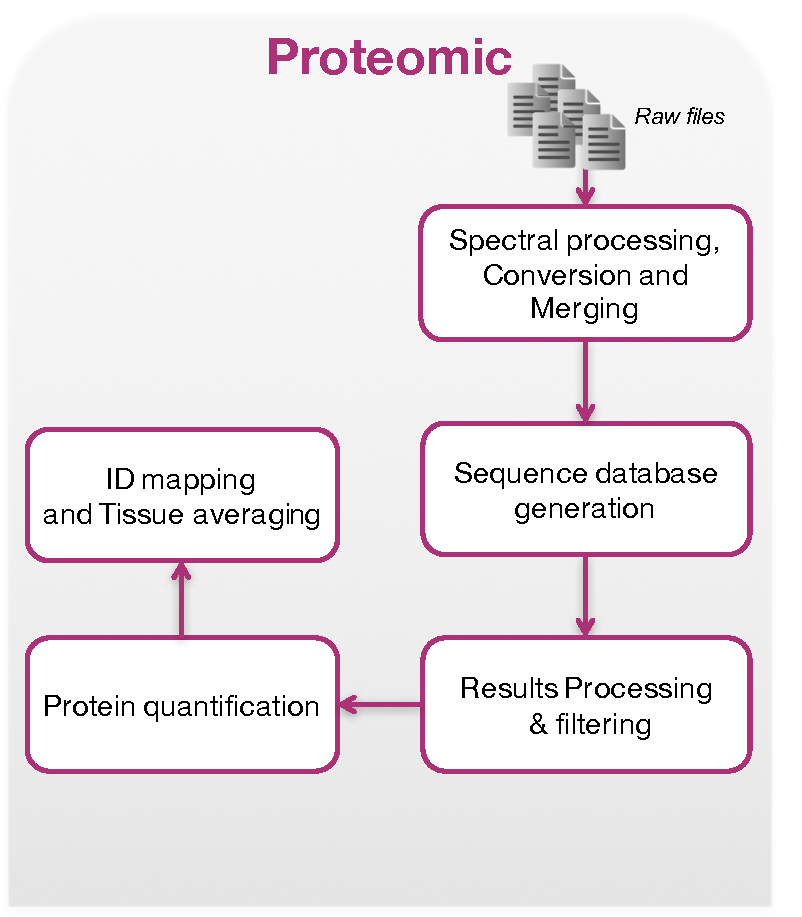
\includegraphics[scale=0.75]{additional/pipelineProteins.pdf}\centering
      \caption[General steps for processing the proteome
      data]{\label{fig:pipelineProt}\textbf{General steps for processing the
      proteome} [TK] }
  \end{figure}

